\setcounter{chapter}{8}

\chapter{重积分}

\begin{introduction}
    \item 二重积分
    \item 三重积分
    \item 重积分的应用
\end{introduction}

\section{二重积分}
\textbf{二重积分的概念}

函数$f(x,y)$在二维有界闭区域$D$上的二重积分系指下述和式的极限:
\begin{equation*}
    \iint \limits_{D} f(x,y) f(x,y)\deriv x\deriv y=\lim_{\lambda\rightarrow 0}\sum_{i=1}^n f(\xi_i,\eta_i)\Delta \sigma_i
\end{equation*}
其中$\Delta \sigma_i$是分割区域$D$为$n$个子区域$\sigma_1,\sigma_2,\cdots,\sigma_n$时子区域$\sigma_i$的面积,而$(\xi_i,\eta_i)\in\sigma_i,\lambda$为各子区域$\sigma_i(i=1,2,\cdots,n)$直径之最大者.

\begin{property} \label{property:double_integral}
    \begin{enumerate}
        \item $\displaystyle\iint \limits_{D} kf(x,y)\deriv\sigma=k\iint \limits_{D} f(x,y)\deriv\sigma$,其中$k$为常数
        \item $\displaystyle\iint \limits_{D} [f(x,y)\pm g(x,y)]\deriv\sigma=\iint \limits_{D} f(x,y)\deriv\sigma\pm\iint \limits_{D} g(x,y)\deriv\sigma$
        \item 若有界闭区域$D$能分为两个闭区域$D_1$和$D_2$,则
        \begin{equation*}
            \iint \limits_{D} f(x,y)\deriv\sigma=\iint \limits_{D_1} f(x,y)\deriv\sigma+\iint \limits_{D_2} f(x,y)\deriv\sigma
        \end{equation*}
        即二重积分对于积分区域具有可加性
        \item (二重积分的保号性)若在区域$D$上,$f(x,y)\leq\varphi(x,y)$,则
        \begin{equation*}
            \iint \limits_{D} f(x,y)\deriv\sigma\leq\iint \limits_{D} \varphi(x,y)\deriv\sigma
        \end{equation*}
        \item (二重积分的估值定理)设在有界闭区域$D$上$f(x,y)$的最大值和最小值分别为$M$和$m$,则
        \begin{equation*}
            m\sigma\leq\iint \limits_{D} f(x,y)\deriv\sigma\leq M\sigma
        \end{equation*}
        其中$\sigma$是区域$D$的面积
        \item (二重积分的中值定理)设函数$f(x,y)$在有界闭区域$D$上连续,则在$D$上至少存在一点$(\xi,\eta)$,使得
        \begin{equation*}
            \iint \limits_{D} f(x,y)\deriv\sigma=f(\xi,\eta)\sigma
        \end{equation*}
        其中$\sigma$是区域$D$的面积
    \end{enumerate}
\end{property}

\textbf{二重积分计算法}

(1)在直角坐标系中的计算法

在直角坐标系中,二重积分的面积元素$\deriv\sigma$可写成$\deriv x\deriv y$,于是
\begin{equation*}
    \iint \limits_{D} f(x,y)\deriv\sigma=\iint \limits_{D} f(x,y)\deriv x\deriv y
\end{equation*}

如果积分区域$D$是由两条直线$x=a,x=b$与两条曲线$y=\varphi_1(x),y=\varphi_2(x)$所围成(如图\ref{p9_1_1}所示)\\
即
\begin{equation*}
    D:
    \begin{cases}
        a \leq x \leq b \\
        \varphi_1(x) \leq y \leq \varphi_2(x)
    \end{cases}
\end{equation*}
则
\begin{equation*}
    \iint \limits_{D} f(x,y)\deriv x\deriv y=\int_{a}^{b}\deriv x \int_{\varphi_1(x)}^{\varphi_2(x)} f(x,y)\deriv y
\end{equation*}

如果积分区域$D$是由两条直线$y=c,y=d$与两条曲线$x=\psi_1(y),x=\psi_2(y)$所围成(如图\ref{p9_1_2}所示)\\
即
\begin{equation*}
    D:
    \begin{cases}
        c \leq y \leq d \\
        \psi_1(y) \leq x \leq \psi_2(y)
    \end{cases}
\end{equation*}
则
\begin{equation*}
    \iint \limits_{D} f(x,y)\deriv x\deriv y=\int_{c}^{d}\deriv y \int_{\psi_1(y)}^{\psi_2(y)} f(x,y)\deriv x
\end{equation*}

\begin{figure}[H]
	\centering
	\begin{minipage}{0.49\linewidth}
		\centering
        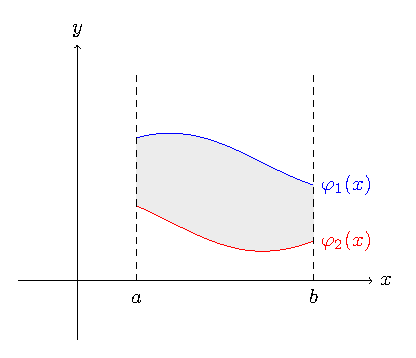
\includegraphics{figure/p9_1_1.pdf}
        \caption{}
        \label{p9_1_1}
		
	\end{minipage}
	\begin{minipage}{0.49\linewidth}
		\centering
		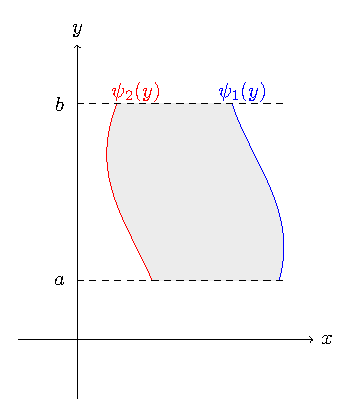
\includegraphics{figure/p9_1_2.pdf}
        \caption{}
        \label{p9_1_2}
	\end{minipage}
	% \caption{ACF and PACF Plots for USA and China}
	% \label{ACF_PACF}
\end{figure}

(2)在极坐标系中的计算法

在极坐标系中$\left\{\begin{aligned} & x=r\cos\theta \\ & y=r\sin\theta \end{aligned}\right.$,面积元素$\deriv\sigma=r\deriv r\deriv\theta$.

如果极点$O$不在区域$D$上,而区域$D$是由两条射线$\theta=\alpha,\theta=\beta$与两条曲线$r=r_1(\theta),r=r_2(\theta)$所围成(如图\ref{p9_1_3}所示)\\
即
\begin{equation*}
    D:
    \begin{cases}
        \alpha \leq \theta \leq \beta \\
        r_1(\theta) \leq r \leq r_2(\theta)
    \end{cases}
\end{equation*}
则
\begin{equation*}
    \iint \limits_{D} f(x,y)\deriv\sigma=\int_{\alpha}^{\beta}\deriv\theta \int_{r_1(\theta)}^{r_2(\theta)} f(r\cos\theta,r\sin\theta)r\deriv r
\end{equation*}

如果区域$D$是曲边扇形(如图\ref{p9_1_4}所示),\\
即
\begin{equation*}
    D:
    \begin{cases}
        \alpha \leq \theta \leq \beta \\
        0 \leq r \leq r(\theta)
    \end{cases}
\end{equation*}
则
\begin{equation*}
    \iint \limits_{D} f(x,y)\deriv\sigma=\int_{\alpha}^{\beta}\deriv\theta \int_{0}^{r(\theta)} f(r\cos\theta,r\sin\theta)r\deriv r
\end{equation*}

如果区域$D$是由闭曲线$r=r(\theta)$所围成,且极点$O$在区域$D$内(如图\ref{p9_1_5}所示),\\
则
\begin{equation*}
    \iint \limits_{D} f(x,y)\deriv\sigma=\int_{0}^{2\pi}\deriv\theta \int_{0}^{r(\theta)} f(r\cos\theta,r\sin\theta)r\deriv r
\end{equation*}

\begin{figure}[H]
	\centering
	\begin{minipage}{0.49\linewidth}
		\centering
        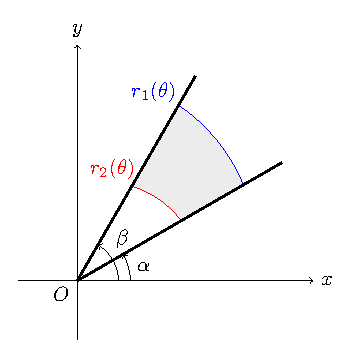
\includegraphics[width=6cm]{figure/p9_1_3.pdf}
        \caption{}
        \label{p9_1_3}
	\end{minipage}
	\begin{minipage}{0.49\linewidth}
		\centering
		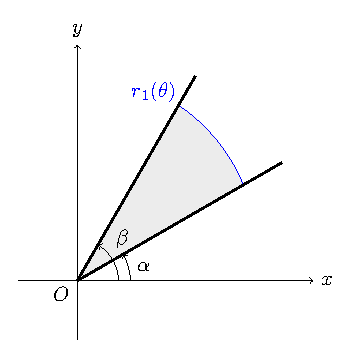
\includegraphics[width=6cm]{figure/p9_1_4.pdf}
        \caption{}
        \label{p9_1_4}
	\end{minipage}

    \begin{minipage}{0.3\linewidth}
		\centering
		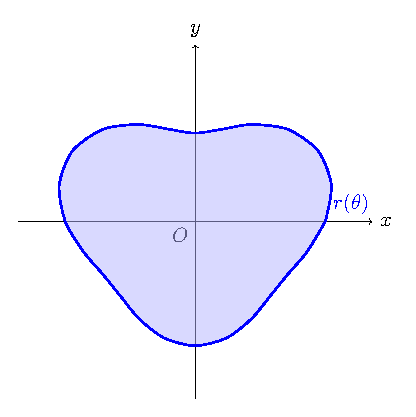
\includegraphics[width=6cm]{figure/p9_1_5.pdf}
        \caption{}
        \label{p9_1_5}
	\end{minipage}
	% \caption{ACF and PACF Plots for USA and China}
	% \label{ACF_PACF}
\end{figure}

\textbf{二重积分的普通对称性与轮换对称性}

\textbf{(1)普通对称性}

若积分区域$D$关于$y$轴对称,则
\begin{equation*}
    \iint \limits_{D} f(x,y)\deriv x\deriv y=
    \begin{cases}
        2\displaystyle\iint \limits_{D_1} f(x,y)\deriv x\deriv y, \quad & f(x,y)=f(-x,y) \\
        0,  & f(x,y)=-f(-x,y)
    \end{cases}
\end{equation*}
其中$D_1$是$D$关于$y$轴的右半部分.

若积分区域$D$关于$x$轴对称,则
\begin{equation*}
    \iint \limits_{D} f(x,y)\deriv x\deriv y=
    \begin{cases}
        2\displaystyle\iint \limits_{D_1} f(x,y)\deriv x\deriv y, \quad & f(x,y)=f(x,-y) \\
        0,  & f(x,y)=-f(x,-y)
    \end{cases}
\end{equation*}
其中$D_1$是$D$关于$x$轴的上半部分.

\textbf{(2)轮换对称性}

若把$x$与$y$对调后,区域$D$不变(或区域$D$关于$y=x$对称),则
\begin{equation*}
    \iint \limits_{D} f(x,y)\deriv x\deriv y=\iint \limits_{D} f(y,x)\deriv x\deriv y=\dfrac{1}{2}\iint \limits_{D} [f(x,y)+f(y,x)]\deriv x\deriv y
\end{equation*}

\section{三重积分}
\textbf{三重积分的概念}

函数$f(x,y,z)$在三维有界闭区域上$\Omega$上的三重积分系指下述和式的极限:
\begin{equation*}
    \iiint \limits_{\Omega} f(x,y,z)\deriv x\deriv y\deriv z=\lim_{\lambda\rightarrow 0}\sum_{i=1}^n f(\xi_i, \eta_i, \zeta_i)\Delta V_i
\end{equation*}
其中$\Delta V_i$是分割区域$\Omega$为$n$个子区域$V_1,V_2,\cdots,V_n$时子区域$V_i$的体积,而$(\xi_i, \eta_i, \zeta_i)\in V_i$,$\lambda$为各子区域$V_i(i=1,2,\cdots,n)$直径之最大者.

若$f(x,y,z)$在$\Omega$上连续,则上述三重积分存在.

\textbf{三重积分的计算法}

(1)在直角坐标系中的计算法

在直角坐标系中,三重积分的体积元素$\deriv V$为$\deriv x\deriv y\deriv z$。设空间有界闭区域$\Omega$在$xOy$平面上的投影为$D_{xy}$,且平行于$z$轴的直线与$\Omega$的边界曲面$S$的交点不多于两个。此时如果$\Omega$可表示为
\begin{equation*}
    \Omega:
    \begin{cases}
        a \leq x \leq b \\
        y_1(x) \leq y \leq y_2(x) \\
        z_1(x,y) \leq z \leq z_2(x,y)
    \end{cases}
\end{equation*}
则
\begin{align*}
    & \iiint \limits_{\Omega} f(x,y,z)\deriv V = \iiint \limits_{\Omega} f(x,y,z)\deriv x\deriv y\deriv z \\
    = & \iint \limits_{D_{xy}}\deriv x\deriv y\int_{z_1(x,y)}^{z_2(x,y)} f(x,y,z)\deriv z = \int_{a}^{b}\deriv x \int_{y_1(x)}^{y_2(x)}\deriv y \int_{z_1(x,y)}^{z_2(x,y)} f(x,y,z)\deriv z
\end{align*}

(2)在柱面坐标系下的计算法

直角坐标与柱面坐标的关系是 \quad $\left\{\begin{aligned} & x=r\cos\theta \\ & y=r\sin\theta \\ & z=z\end{aligned}\right.$\\
在柱面坐标系中三重积分的体积元素$\deriv V$为$r\deriv r\deriv\theta\deriv z$,因此
\begin{equation*}
    \iiint \limits_{\Omega} f(x,y,z)\deriv V = \iiint \limits_{\Omega} f(r\cos\theta,r\sin\theta,z)r\deriv r\deriv\theta\deriv z
\end{equation*}
将右端化为累次积分,即可求得其结果.

(3)在球面坐标系下的计算法

直角坐标与球面坐标的关系是 \quad $\left\{\begin{aligned} & x=r\sin\varphi\cos\theta \\ & y=r\sin\varphi\sin\theta \\ & z=r\cos\varphi\end{aligned}\right.$\\
在球面坐标系中三重积分的体积元素$\deriv V$为$r^2\sin\varphi\deriv r\deriv\varphi\deriv\theta$,因此
\begin{equation*}
    \iiint \limits_{\Omega} f(x,y,z)\deriv V = \iiint \limits_{\Omega} f(r\sin\varphi\cos\theta,r\sin\varphi\sin\theta,r\cos\varphi)r^2\sin\varphi\deriv r\deriv\varphi\deriv\theta
\end{equation*}
将右端化为累次积分,即可求得其结果.

\textbf{三重积分的普通对称性和轮换对称性}

\textbf{(1)普通对称性}

若积分区域$\Omega$关于$yOz$面对称,则
\begin{equation*}
    \iiint \limits_{\Omega} f(x,y,z)\deriv v=
    \begin{cases}
        2\displaystyle\iiint \limits_{\Omega_1} f(x,y,z)\deriv v, \quad & f(x,y,z)=f(-x,y,z) \\
        0,  & f(x,y,z)=-f(-x,y,z)
    \end{cases}
\end{equation*}
其中$\Omega_1$是$\Omega$在$yOz$面前面的部分.

关于其他坐标面对称的情况与此类似

\textbf{(2)轮换对称性}

若把$x$与$y$对调后,$\Omega$不变,则$\displaystyle\iiint\limits_{\Omega}f(x,y,z)\deriv v=\iiint\limits_{\Omega}f(y,x,z)$

关于其他情况与此类似

如$\Omega=\{(x,y,z)|x^2+y^2+z^2\leq R^2\}$,则$\displaystyle\iiint\limits_{\Omega}f(x)\deriv v=\iiint\limits_{\Omega}f(y)\deriv v=\iiint\limits_{\Omega}f(z)\deriv v$可以化简计算.

\section{重积分的应用}

\textbf{1.计算面积}

(1)平面闭域面积为$\displaystyle A=\iint \limits_{D} \deriv x\deriv y$

(2)设曲面$\Sigma$的方程为$z=f(x,y)$,$\Sigma$在$xOy$平面上投影区域为$D$,$f(x,y)$在$D$上存在连续偏导数,则曲面$\Sigma$的面积为
\begin{equation*}
    A=\iint \limits_{D} \sqrt{1+\left(\dfrac{\partial z}{\partial x}\right)^2+\left(\dfrac{\partial z}{\partial y}\right)^2}\deriv x\deriv y
\end{equation*}

\textbf{2.计算体积}

(1)曲顶柱体的体积 \quad 设柱体上顶是连续的曲面$z=f(x,y)((x,y)\in D,f(x,y)\geq 0)$,下底是平面$z=0$,侧面为以区域$D$的边界曲线为准线而母线平行于$z$轴的柱面,则此柱体的体积为
\begin{equation*}
    V=\iint \limits_{D} f(x,y)\deriv x\deriv y
\end{equation*}

(2)已知边界曲面的空间区域$\Omega$的体积 \quad $V=\displaystyle\iiint \limits_{\Omega}\deriv x\deriv y\deriv z$